% Copyright 2004 by Till Tantau <tantau@users.sourceforge.net>.
%
% In principle, this file can be redistributed and/or modified under
% the terms of the GNU Public License, version 2.
%
% However, this file is supposed to be a template to be modified
% for your own needs. For this reason, if you use this file as a
% template and not specifically distribute it as part of a another
% package/program, I grant the extra permission to freely copy and
% modify this file as you see fit and even to delete this copyright
% notice. 

\documentclass{beamer}

% There are many different themes available for Beamer. A comprehensive
% list with examples is given here:
% http://deic.uab.es/~iblanes/beamer_gallery/index_by_theme.html
% You can uncomment the themes below if you would like to use a different
% one:
%\usetheme{AnnArbor}
%\usetheme{Antibes}
%\usetheme{Bergen}
%\usetheme{Berkeley}
%\usetheme{Berlin}
%\usetheme{Boadilla}
%\usetheme{boxes}
%\usetheme{CambridgeUS}
%\usetheme{Copenhagen}
%\usetheme{Darmstadt}
%\usetheme{default}
%\usetheme{Frankfurt}
%\usetheme{Goettingen}
%\usetheme{Hannover}
%\usetheme{Ilmenau}
%\usetheme{JuanLesPins}
%\usetheme{Luebeck}
\usetheme{Madrid}
%\usetheme{Malmoe}
%\usetheme{Marburg}
%\usetheme{Montpellier}
%\usetheme{PaloAlto}
%\usetheme{Pittsburgh}
%\usetheme{Rochester}
%\usetheme{Singapore}
%\usetheme{Szeged}
%\usetheme{Warsaw}


% Customize Warsaw color 
\setbeamercolor*{palette primary}{use=structure,fg=white,bg=red!50!black}
\setbeamercolor*{palette secondary}{use=structure,fg=white,bg=red!60!black}
\setbeamercolor*{palette tertiary}{use=structure,fg=white,bg=red!70!black}

% Customize Warsaw block title and background colors
\setbeamercolor{block title}{bg=red!50!black,fg=white}


% List your packages here

\usepackage[colorinlistoftodos]{todonotes}
\usepackage{media9}

\title[DC Motor Progress]{BEMOSS and Its Enhanced Applications}

% % A subtitle is optional and this may be deleted
% \subtitle{Product Proposal}

\author[B.~Lauer]{Brian~Lauer \\\and
Advisor: Dr. Suruz Miah}
% - Give the names in the same order as the appear in the paper.
% - Use the \inst{?} command only if the authors have different
%   affiliation.

\institute[Bradley University] % (optional, but mostly needed)
{
  Department of Electrical and Computer Engineering\\
  Bradley University\\
  1501 W. Bradley Avenue\\
  Peoria, IL, 61625, USA
}
% - Use the \inst command only if there are several affiliations.
% - Keep it simple, no one is interested in your street address.

\date[July~19,~2019]{Friday, July~19,~2019}
% - Either use conference name or its abbreviation.
% - Not really informative to the audience, more for people (including
%   yourself) who are reading the slides online

\logo{\hfill\href{http://www.bradley.edu}{
\includegraphics[width=0.75cm]{figs/logoBU1-Print}}}  % place logo in every page 


\subject{Mobile Robot Localization}
% This is only inserted into the PDF information catalog. Can be left
% out. 

% If you have a file called "university-logo-filename.xxx", where xxx
% is a graphic format that can be processed by latex or pdflatex,
% resp., then you can add a logo as follows:

% \pgfdeclareimage[height=0.5cm]{university-logo}{university-logo-filename}
% \logo{\pgfuseimage{university-logo}}

% Delete this, if you do not want the table of contents to pop up at
% the beginning of each subsection:

% Let's get started
\begin{document}

\begin{frame}
  \titlepage
\end{frame}

\begin{frame}{Outline}
  \tableofcontents
  % You might wish to add the option [pausesections]
\end{frame}

\section{Current Motor Interface}

\begin{frame}{Current Motor Interface}{}
	\begin{itemize}
		\item Using command \texttt{nmap -sn 192.168.1.0/24} to perform ping scan
		\item Command \texttt{arp -a} dumps ARP (Address Resolution Protocol) cache
		\item Unable to use command \texttt{sudo nmap -sn 192.168.1.0/24}
		\item User input not accepted in VOLTTRON log terminal
	\end{itemize}
\end{frame}

\begin{frame}{Current Motor Interface}{}
	\begin{figure}
		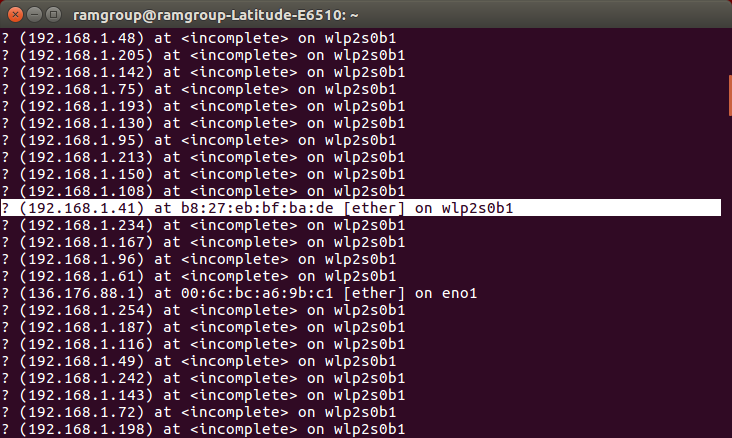
\includegraphics[scale=0.4]{figs/arpoutput.png}
		\caption{Use of \texttt{arp} command}
	\end{figure}
\end{frame}

\begin{frame}{Current Motor Interface}{}
	\begin{itemize}
		\item Parse arp output with regex
		\item Retrieve IP and mac address of Raspberry Pi
		\item Remove \texttt{':'} delimiters from MAC address
		\item Regex in URL mapping to \texttt{devicedata\_view} only searches for \texttt{a-z}, \texttt{A-Z}, and \texttt{0-9}
	\end{itemize}
\end{frame}

\subsection{Problems}

\begin{frame}{Current Motor Interface}{Problems}
	\begin{itemize}
		\item Device model, vendor name, username, and password of Pi not easily accessible
		\item Hardcoded in json file
		\item Password must be encrypted 
		\item RPi script paths must be specified on BEMOSS host machine
	\end{itemize}
\end{frame}

\subsection{Demo}

\begin{frame}{Current Motor Interface}{Demo}
\center
Play video
\end{frame}

\section{Improved Motor Interface}

\begin{frame}{Improved Motor Interface}{}
	\begin{itemize}
		\item Raspberry Pi remote GPIO server
		\item Control GPIO pins over the Internet
		\item gpiozero or pigpio python libraries
		\item Only requires IP address, no login credentials
	\end{itemize}
\end{frame}

\section{Plans}

\begin{frame}{Plans}{}
	\begin{itemize}
		\item Find new device to implement with BEMOSS
		\item Implement PID control algorithm with motor to control speed
	\end{itemize}
\end{frame}

%\section{
% You can reveal the parts of a slide one at a time
% with the \pause command:
%\begin{frame}{Second Slide Title}
%  \begin{itemize}
%  \item {
%    First item.
%    \pause % The slide will pause after showing the first item
%  }
  %\item {   
  %  Second item.
 % }
  % You can also specify when the content should appear
  % by using <n->:
 % \item<3-> {
 %   Third item.
 % }
%  \item<4-> {
%    Fourth item.
 % }
  % or you can use the \uncover command to reveal general
  % content (not just \items):
%  \item<5-> {
%    Fifth item. \uncover<6->{Extra text in the fifth item.}
%  }
%  \end{itemize}
%\end{frame}

%\section{Second Main Section}

%\subsection{Another Subsection}

%\begin{frame}{Blocks}
%\begin{block}{Block Title}
%You can also highlight sections of your %presentation in a block, with it's own %title
%\end{block}
%\begin{theorem}
%There are separate environments for %theorems, examples, definitions and proofs.
%\end{theorem}
%\begin{example}
%Here is an example of an example block.
%\end{example}
%\end{frame}

% Placing a * after \section means it will not show in the
% outline or table of contents.
% All of the following is optional and typically not needed. 
\begin{frame}
	\centering
	Any questions?
\end{frame}

\end{document}



%%% Local Variables:
%%% mode: latex
%%% TeX-master: t
%%% End:
